\documentclass[11pt]{article}
\usepackage[margin=1in]{geometry}
\usepackage{xcolor}
\usepackage{tcolorbox}
\usepackage{enumitem}
\usepackage{fontawesome5}
\usepackage{titlesec}
\usepackage{multicol}
\usepackage{tikz}
\usepackage{fancyhdr}
\usepackage{lastpage}

% Color definitions
\definecolor{noirblack}{RGB}{25, 25, 25}
\definecolor{rainblue}{RGB}{70, 130, 180}
\definecolor{neongreen}{RGB}{50, 205, 50}
\definecolor{bloodred}{RGB}{178, 34, 34}
\definecolor{smokegrey}{RGB}{105, 105, 105}
\definecolor{goldaccent}{RGB}{218, 165, 32}
\definecolor{streetlamp}{RGB}{255, 215, 0}
\definecolor{vicepurple}{RGB}{128, 0, 128}

% Box styles
\tcbset{
    noirbox/.style={
        enhanced,
        colback=white,
        colframe=#1,
        arc=0pt,
        fonttitle=\bfseries,
        before skip=10pt,
        after skip=10pt,
        boxrule=1pt
    }
}

\newtcolorbox{noirsection}[2][]{%
    noirbox=#2,
    title=#1
}

\titleformat{\section}{\color{noirblack}\Large\bfseries\filcenter}{}{0em}{}
\titleformat{\subsection}{\color{smokegrey}\large\bfseries}{}{0em}{}

\setlist{left=0pt}

% Header and footer
\pagestyle{fancy}
\fancyhf{}
\rhead{Modern Noir Campaign}
\lhead{Neon Shadows}
\rfoot{Page \thepage\ of \pageref{LastPage}}
\lfoot{Fate's Edge Expansion}

\title{\Huge\textbf{Neon Shadows}\\
\Large A Modern Noir Expansion for Fate's Edge\\
\large Optimized for Quick Sessions}
\author{}
\date{}

\begin{document}

\maketitle

\begin{center}
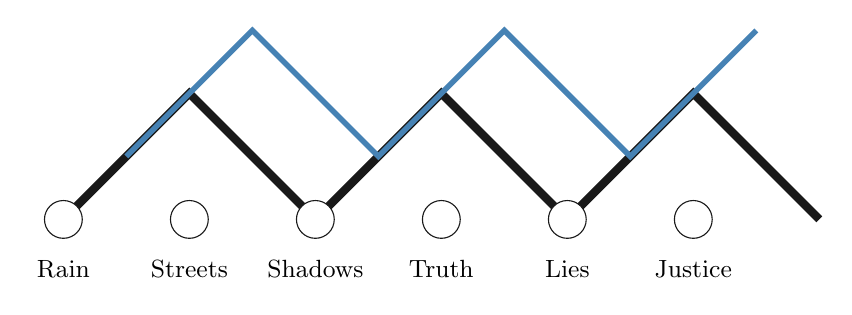
\begin{tikzpicture}[scale=0.8]
\draw[noirblack, line width=3pt] (0,0) -- (2,2) -- (4,0) -- (6,2) -- (8,0) -- (10,2) -- (12,0);
\draw[rainblue, line width=2pt] (1,1) -- (3,3) -- (5,1) -- (7,3) -- (9,1) -- (11,3);
\foreach \x/\name in {0/Rain, 2/Streets, 4/Shadows, 6/Truth, 8/Lies, 10/Justice} {
    \draw[noirblack, fill=white] (\x,0) circle (0.3cm);
    \node[below, font=\small] at (\x,-0.5) {\name};
}
\end{tikzpicture}
\end{center}

\begin{noirsection}[Campaign Overview]{noirblack}
\subsection*{\faMap\ Campaign Hook}

\textbf{The Premise:} You are a private investigator, detective, or troubled professional working the mean streets of a modern city where neon lights cast long shadows and everyone has something to hide. The cases are personal, the stakes are high, and the truth is rarely simple.

\textbf{Real Hook:} In a city where corruption runs deep and justice is often just another commodity, you've chosen to walk the line between order and chaos. But every case you take pulls you deeper into a web of lies, and every truth you uncover makes you a target.

\textbf{Thematic Elements:} Moral Ambiguity, Urban Decay, Personal Stakes, Information As Currency, Noir Atmosphere

\textbf{Key Noir Elements:}
\begin{itemize}
    \item \textbf{Moral Ambiguity:} Right and wrong are not clearly defined
    \item \textbf{Urban Isolation:} Characters are alone in a crowded city
    \item \textbf{Information Control:} Knowledge is power, and everyone guards theirs carefully
    \item \textbf{Personal Consequences:} Choices have lasting impact on character and story
    \item \textbf{Atmospheric Tension:} Mood and setting drive the narrative as much as plot
\end{itemize}
\end{noirsection}

\newpage

\section{Quick Case System}

\subsection*{\faFolder\ Core Investigation Mechanics}

\textbf{One-Shot Case Framework (Designed for 2-3 hour sessions):}

\textbf{Case Elements (Draw 3 cards from standard deck):}
\begin{itemize}
    \item \textbf{Spade:} Crime/Inciting Incident (the hook that pulls you in)
    \item \textbf{Heart:} Key Person (central figure in the case)
    \item \textbf{Club:} Complication/Pressure (what makes it difficult)
    \item \textbf{Diamond:} Reward/Resolution (what you can gain or achieve)
\end{itemize}

\textbf{Rank Interpretation:}
\begin{itemize}
    \item \textbf{2-5:} Simple case with straightforward resolution
    \item \textbf{6-10:} Moderate complexity with meaningful choices
    \item \textbf{J/Q/K:} Complex case with multiple viable solutions
    \item \textbf{Ace:} Twist - the case is not what it initially seemed
\end{itemize}

\textbf{Quick Setup:}
\begin{enumerate}
    \item Draw 3 cards (Spade, Heart, Club)
    \item Identify the highest rank as your main Challenge Clock (2-5: 4 segments, 6-10: 6 segments, J/Q/K: 8 segments, A: 10 segments)
    \item Start with 2 Investigation Points
\end{enumerate}

\textbf{Core investigative activities (use Fate's Edge core mechanic):}

\textbf{Surveillance (Wits + Stealth, DV 2-4):}
\begin{itemize}
    \item Following suspects without detection
    \item Observing meetings and transactions
    \item Gathering behavioral intelligence
\end{itemize}

\textbf{Interview (Presence + Insight, DV 1-3):}
\begin{itemize}
    \item Direct questioning of witnesses and suspects
    \item Reading body language and micro-expressions
    \item Building rapport or applying pressure
\end{itemize}

\textbf{Research (Wits + Investigation, DV 2-3):}
\begin{itemize}
    \item Database searches and record checks
    \item Background investigations on persons of interest
    \item Cross-referencing information for patterns
\end{itemize}

\textbf{Scene Examination (Wits + Perception, DV 1-4):}
\begin{itemize}
    \item Physical evidence collection and analysis
    \item Crime scene reconstruction
    \item Pattern recognition in evidence placement
\end{itemize}

\textbf{Infiltration (Wits + Subterfuge, DV 3-4):}
\begin{itemize}
    \item Gaining access to restricted locations
    \item Undercover operations
    \item Social engineering and deception
\end{itemize}

\textbf{Investigation Points:} Spend 1 point to automatically succeed on any investigation action once per scene

\textbf{Evidence Rating System:}
\begin{itemize}
    \item \textbf{A+ Evidence:} Unimpeachable - direct observation, clear documentation, multiple witnesses
    \item \textbf{A Evidence:} Strong - solid documentation, reliable witness, clear chain of custody
    \item \textbf{B Evidence:} Good - circumstantial but compelling, single reliable witness
    \item \textbf{C Evidence:} Fair - circumstantial, questionable witness reliability
    \item \textbf{D Evidence:} Weak - hearsay, speculation, compromised source
    \item \textbf{F Evidence:} Unreliable - contradicted, obtained illegally, severely compromised
\end{itemize}

\textbf{Evidence Degradation:} Each day without follow-up reduces evidence quality by one grade
\end{section}

\newpage

\section{Vice Clock System}

\subsection*{\faHeartBroken\ Personal Demons}

\textbf{Core Concept:}
The Vice Clock represents your character's ongoing struggle with personal demons that threaten to undermine their professional life and moral compass. It's a mechanical representation of the noir protagonist's fatal flaw.

\textbf{Vice Clock Structure:}
\begin{itemize}
    \item \textbf{4-Segment Clock:} Visual tracker that increments during play
    \item \textbf{Increments:} +1 segment per scene (automatic unless prevented)
    \item \textbf{Prevention:} Spend 1 Boon to stop increment in that scene
    \item \textbf{Resolution:} Spend 2 Boons to clear 1 segment
\end{itemize}

\textbf{16-Card Vice Deck (Face Cards Only):}

\textbf{Hearts (Emotional Vice) - Red:}
\begin{itemize}
    \item \textbf{Jack:} "She's Trouble" - Compulsive contact with toxic relationships
    \item \textbf{Queen:} "Lover's Betrayal" - Romantic entanglements that compromise work
    \item \textbf{King:} "Obsessive Pursuit" - Inability to let go of personal cases
    \item \textbf{Ace:} "Love Conquers All" - Catastrophic sacrifice for unworthy causes
\end{itemize}

\textbf{Spades (Physical Vice) - Black:}
\begin{itemize}
    \item \textbf{Jack:} "Nightcap" - Drinking affects performance and sleep
    \item \textbf{Queen:} "Hard Liquor" - Regular substance abuse impacts health
    \item \textbf{King:} "Bottle Courage" - Need substances for dangerous situations
    \item \textbf{Ace:} "Rock Bottom" - Overdose, withdrawal, or violent episodes
\end{itemize}

\textbf{Clubs (Professional Vice) - Black:}
\begin{itemize}
    \item \textbf{Jack:} "Bent Rules" - Cutting corners attracts official scrutiny
    \item \textbf{Queen:} "Dirty Deals" - Taking bribes or compromising ethics
    \item \textbf{King:} "Corrupt Core" - Systematic abuse of professional position
    \item \textbf{Ace:} "Badge of Corruption" - Authority weaponized for personal gain
\end{itemize}

\textbf{Diamonds (Psychological Vice) - Red:}
\begin{itemize}
    \item \textbf{Jack:} "Paranoid Tendencies" - Seeing threats, alienating allies
    \item \textbf{Queen:} "Trust Issues" - Inability to work effectively with others
    \item \textbf{King:} "Complete Isolation" - No personal connections, vulnerable
    \item \textbf{Ace:} "Psychotic Break" - Hallucinations, delusions, blackouts
\end{itemize}

\textbf{Vice Clock States:}

\textbf{1 Segment - Temptation:}
\begin{itemize}
    \item Generate 1 additional CP when rolling for actions related to this vice
    \item Minor roleplay reminders (character references the temptation)
\end{itemize}

\textbf{2 Segments - Habit:}
\begin{itemize}
    \item Generate 2 additional CP when rolling for vice-related actions
    \item -1 die penalty to rolls when resisting the vice
    \item Start scenes with 1 banked CP related to this vice
\end{itemize}

\textbf{3 Segments - Addiction:}
\begin{itemize}
    \item Generate 3 additional CP when rolling for vice-related actions
    \item -2 dice penalty to rolls when resisting or when deprived
    \item Must spend 1 Boon per session just to function normally
    \item Start scenes with 2 banked CP related to this vice
\end{itemize}

\textbf{4 Segments - Crisis:}
\begin{itemize}
    \item Generate 4 additional CP when rolling for vice-related actions
    \item -3 dice penalty to ALL rolls when deprived
    \item Cannot spend Boons for other benefits until crisis resolved
    \item Start scenes with 3 banked CP related to this vice
\end{itemize}

\textbf{Vice Clock Management:}

\textbf{Prevention (Ongoing):}
\begin{itemize}
    \item \textbf{Cost:} 1 Boon per scene
    \item \textbf{Effect:} Prevent Vice Clock from incrementing
\end{itemize}

\textbf{Mitigation (Active):}
\begin{itemize}
    \item \textbf{Cost:} 2 Boons
    \item \textbf{Effect:} Clear 1 segment from Vice Clock
\end{itemize}

\textbf{Escalation (When Full):}
\begin{enumerate}
    \item Draw new Vice card (same or different suit)
    \item Apply appropriate fallout based on card rank
    \item Reset clock based on new card (Jack=1, Queen=2, King=3, Ace=4)
\end{enumerate}

\textbf{Character Creation Integration:}

\textbf{Starting Vice Clock Values:}
\begin{itemize}
    \item \textbf{Jack Draw:} 1 segment
    \item \textbf{Queen Draw:} 2 segments
    \item \textbf{King Draw:} 3 segments  
    \item \textbf{Ace Draw:} 4 segments (immediate crisis scene)
\end{itemize}

\textbf{Multiple Vice Management:}
\begin{itemize}
    \item Only one Vice Clock increments per scene (character's choice)
    \item Other vices generate 1 CP each per scene regardless
    \item Managing multiple vices requires proportionally more resources
\end{itemize}
\end{section}

\newpage

\section{Quick NPC System}

\subsection*{\faUsers\ Important Characters}

\textbf{The Femme Fatale:}
\begin{itemize}
    \item \textbf{Archetype:} Dangerous woman with hidden agenda
    \item \textbf{Motivation:} Personal gain, revenge, or protection of secrets
    \item \textbf{Methods:} Manipulation, seduction, information control
    \item \textbf{Weakness:} Overconfidence, emotional vulnerability, over-elaborate schemes
    \item \textbf{Red Flags:} Knows more than she should about the case; Appears at crucial moments; Has unexplained wealth or connections; Changes story when pressed
    \item \textbf{Potential Roles:} Client, witness, suspect, ally, or mastermind
\end{itemize}

\textbf{The Corrupt Cop:}
\begin{itemize}
    \item \textbf{Archetype:} Law enforcement officer on the take
    \item \textbf{Motivation:} Money, power, protection from own crimes
    \item \textbf{Methods:} Evidence tampering, witness intimidation, information brokering
    \item \textbf{Weakness:} Paranoia, need for control, predictable routines
    \item \textbf{Red Flags:} Always "conveniently" arrives late to crime scenes; Has unexplained income or expensive tastes; Knows details that weren't in official reports; Pressures investigation in specific directions
    \item \textbf{Potential Roles:} Investigator, suspect, obstruction, or reluctant informant
\end{itemize}

\textbf{The Wealthy Businessman:}
\begin{itemize}
    \item \textbf{Archetype:} Respectable figure with dark secrets
    \item \textbf{Motivation:} Protecting empire, eliminating threats, maintaining image
    \item \textbf{Methods:} Money, influence, legal intimidation, hired muscle
    \item \textbf{Weakness:} Public exposure, legal vulnerabilities, family concerns
    \item \textbf{Red Flags:} Everything seems legitimate on paper; Has connections in high places; Willing to spend large sums to "resolve" problems; Associates with unsavory characters discretely
    \item \textbf{Potential Roles:} Client, victim, suspect, employer, or case originator
\end{itemize}

\textbf{The Broken Veteran:}
\begin{itemize}
    \item \textbf{Archetype:} Former hero fallen on hard times
    \item \textbf{Motivation:} Survival, justice, redemption, or revenge
    \item \textbf{Methods:} Skills from past life, desperation, insider knowledge
    \item \textbf{Weakness:} Trauma, addiction, moral flexibility, isolation
    \item \textbf{Red Flags:} Has skills that don't match current circumstances; Knows too much about specific procedures or locations; Desperate for money but refuses certain jobs; Displays military or specialized training unconsciously
    \item \textbf{Potential Roles:} Informant, suspect, ally, victim, or tragic figure
\end{itemize}

\textbf{The Informed Citizen:}
\begin{itemize}
    \item \textbf{Archetype:} Ordinary person with crucial knowledge
    \item \textbf{Motivation:} Fear, conscience, revenge, or protection of loved ones
    \item \textbf{Methods:} Observation, accidental discovery, personal connection
    \item \textbf{Weakness:} Fear of consequences, incomplete information, personal bias
    \item \textbf{Red Flags:} Sees investigation but won't approach directly; Has information that doesn't fit official narrative; Behaves nervously around certain topics or people; Knows details that suggest personal involvement
    \item \textbf{Potential Roles:} Witness, reluctant informant, accidental victim, or key to breakthrough
\end{itemize}
\end{section}

\newpage

\section{Urban Environment Mechanics}

\subsection*{\faCity\ City as Character}

\textbf{District Atmosphere:}

\textbf{Downtown/Core Business District:}
\begin{itemize}
    \item \textbf{Atmosphere:} Bright lights, busy streets, corporate power
    \item \textbf{Investigation Modifiers:} +1 to Research, -1 to Surveillance
    \item \textbf{Social Modifiers:} +1 to Interview (professional), -1 to Infiltration
    \item \textbf{Hazards:} Security cameras, private security, high visibility
\end{itemize}

\textbf{Waterfront/Docks:}
\begin{itemize}
    \item \textbf{Atmosphere:} Industrial, dangerous, criminal activity
    \item \textbf{Investigation Modifiers:} +1 to Surveillance, -1 to Interview
    \item \textbf{Social Modifiers:} +1 to Intimidation, -2 to Sway
    \item \textbf{Hazards:} Criminal presence, unsafe structures, limited lighting
\end{itemize}

\textbf{Residential/Suburbs:}
\begin{itemize}
    \item \textbf{Atmosphere:} Quiet, family-oriented, community watchful
    \item \textbf{Investigation Modifiers:} +1 to Interview, -1 to Infiltration
    \item \textbf{Social Modifiers:} +1 to Building Rapport, +1 to Research (public records)
    \item \textbf{Hazards:} Nosy neighbors, home security, limited escape routes
\end{itemize}

\textbf{Entertainment District:}
\begin{itemize}
    \item \textbf{Atmosphere:} Neon, nightlife, temporary anonymity
    \item \textbf{Investigation Modifiers:} +1 to Infiltration, -1 to Surveillance
    \item \textbf{Social Modifiers:} +1 to Social Engineering, -1 to Direct Confrontation
    \item \textbf{Hazards:} Crowds, alcohol/drugs, transient population
\end{itemize}

\textbf{Industrial/Warehouse:}
\begin{itemize}
    \item \textbf{Atmosphere:} Dangerous, isolated, heavy machinery
    \item \textbf{Investigation Modifiers:} +1 to Scene Examination, -2 to Interview
    \item \textbf{Social Modifiers:} +2 to Intimidation, -2 to Sway
    \item \textbf{Hazards:} Physical danger, limited escape, noise cover
\end{itemize}

\textbf{Time and Weather Effects:}

\textbf{Time of Day:}
\begin{itemize}
    \item \textbf{Daylight (6 AM - 6 PM):} +1 to Scene Examination, -1 to Surveillance
    \item \textbf{Twilight (6 AM/6 PM - 8 AM/8 PM):} Balanced conditions
    \item \textbf{Night (8 PM - 6 AM):} +1 to Surveillance, -1 to Interview
\end{itemize}

\textbf{Weather Conditions:}
\begin{itemize}
    \item \textbf{Clear:} Standard conditions
    \item \textbf{Rain:} +1 to Surveillance (fewer witnesses), -1 to Scene Examination (evidence washed away)
    \item \textbf{Fog/Heavy Rain:} +2 to Infiltration, -2 to Interview (people stay inside)
    \item \textbf{Snow:} +1 to Tracking, -1 to Chase Scenes
\end{itemize}

\textbf{Quick Environmental Complications (1 CP each):}
\begin{itemize}
    \item Power outage in the area
    \item Traffic accident blocks access routes
    \item Sudden media attention on the case
    \item Unexpected police presence
    \item Witness becomes unavailable
\end{itemize}
\end{section}

\newpage

\section{Quick Combat System}

\subsection*{\faFistRaised\ Violence in the Shadows}

\textbf{Streamlined combat using Fate's Edge core mechanics:}

\textbf{Position Modifiers:}
\begin{itemize}
    \item \textbf{Controlled:} Ambush, superior weapon, high ground (+1 effect)
    \item \textbf{Risky:} Even match, standard conditions (standard resolution)
    \item \textbf{Desperate:} Outnumbered, poor weapon, disadvantaged (-1 effect)
\end{itemize}

\textbf{Common Combat Actions:}
\begin{itemize}
    \item \textbf{Strike (Body + Melee/Brawl, DV 1-3):} Direct physical attack
    \item \textbf{Shoot (Wits + Firearms, DV 2-4):} Ranged attack (distance/cover affects DV)
    \item \textbf{Evade (Wits + Athletics, DV 2-3):} Avoid incoming attack
    \item \textbf{Intimidate (Presence + Command, DV 2-3):} Psychological warfare
\end{itemize}

\textbf{Harm System (Simplified):}
\begin{itemize}
    \item \textbf{Minor (-):} Bruises, scrapes (1 CP on next 2 rolls)
    \item \textbf{Moderate (=):} Cuts, sprains (1 CP next roll, -1 die)
    \item \textbf{Severe ():} Broken bones, deep cuts (2 CP next roll, -2 dice)
    \item \textbf{Critical (†):} Life-threatening (3 CP next roll, out of action)
\end{itemize}

\textbf{Quick Escalation:} Each 1 rolled in combat generates 1 CP that can be spent immediately by GM for:
\begin{itemize}
    \item Reinforcements arrive (+1 Pressure Clock segment)
    \item Environment becomes hazardous (start Environmental Collapse clock)
    \item Weapon malfunction (attacker suffers -1 die)
    \item Unexpected betrayal (ally becomes hostile)
\end{itemize}
\end{section}

\newpage

\section{Sample Quick Cases}

\subsection*{\faLightbulb\ Ready-to-Run Scenarios}

\textbf{The Missing Heirloom:}
\begin{itemize}
    \item \textbf{Spade 7 (Crime):} A priceless family heirloom was stolen from a locked safe during a charity gala
    \item \textbf{Heart Q (Key Person):} The wealthy socialite whose family owns the item
    \item \textbf{Club 9 (Complication):} Multiple suspects had access, and the family has dark secrets they'd kill to protect
    \item \textbf{Diamond 6 (Reward):} Substantial finder's fee plus access to exclusive social circles
    \item \textbf{Clock:} 6 segments (media attention will ruin the family's reputation)
    \item \textbf{Quick Hook:} "Mrs. Blackwood's emerald necklace disappeared sometime between 9 and 11 PM. The safe was locked, the room was secured, but the necklace is gone. The family is desperate to recover it before tomorrow's society pages."
    \item \textbf{Investigation Points:} Interview the butler, examine the safe for tampering, review security footage
    \item \textbf{Vice Clock Integration:} If investigating involves a romantic interest (Heart Q), players with Emotional Vice may face temptation. If family secrets involve corruption, Professional Vice players may be tempted.
\end{itemize}

\textbf{The Blackmailer:}
\begin{itemize}
    \item \textbf{Spade J (Crime):} Someone is threatening to expose a city councilman's affair unless paid
    \item \textbf{Heart 8 (Key Person):} The councilman's assistant who may know more than she's telling
    \item \textbf{Club K (Complication):} The blackmailer has connections in the police department
    \item \textbf{Diamond 10 (Reward):} The councilman will pay handsomely to end this quietly
    \item \textbf{Clock:} 8 segments (exposure will end the councilman's career and marriage)
    \item \textbf{Quick Hook:} "Councilman Harris has been receiving threatening letters demanding \$50,000. He's desperate but refuses to go to the police. Someone knows his secret and is willing to destroy him for money."
    \item \textbf{Investigation Points:} Trace the letters' origin, interview the councilman's staff, check financial records
    \item \textbf{Vice Clock Integration:} Players with Professional Vice may be tempted by the councilman's offer. Those with Emotional Vice may develop feelings for the assistant.
\end{itemize}

\textbf{The Vanishing Witness:}
\begin{itemize}
    \item \textbf{Spade A (Crime):} A key witness in a murder trial has disappeared the night before testimony
    \item \textbf{Heart 3 (Key Person):} The witness's roommate who claims to know nothing
    \item \textbf{Club 5 (Complication):} The witness owed money to dangerous people
    \item \textbf{Diamond 7 (Reward):} The DA's office will provide protection and a substantial reward
    \item \textbf{Clock:} 6 segments (the trial starts tomorrow and will collapse without the witness)
    \item \textbf{Quick Hook:} "Maria Santos was supposed to testify against the Torrino crime family tomorrow. She didn't show up for work this morning, and her apartment shows signs of a struggle. The prosecution's case will fall apart without her."
    \item \textbf{Investigation Points:} Search the apartment for clues, interview neighbors, check financial records
    \item \textbf{Vice Clock Integration:} Players with Psychological Vice may become paranoid about the danger. Those with Physical Vice may turn to substances under pressure.
\end{itemize}
\end{section}

\newpage

\section{Quick Session Framework}

\subsection*{\faClock\ 3-Hour Session Structure}

\textbf{Designed for maximum noir impact in minimal time:}

\textbf{Opening (30 minutes):}
\begin{enumerate}
    \item Quick character check-in (any updates to relationships/resources?)
    \item Case presentation (3-card draw, explain the hook)
    \item Initial investigation setup (2 Investigation Points, identify first lead)
    \item Vice Clock status check (any increments this session?)
\end{enumerate}

\textbf{Middle (90 minutes):}
\begin{itemize}
    \item 3-4 investigation scenes using core actions
    \item 1-2 social encounters with key NPCs
    \item 1 combat encounter if violence erupts
    \item Advance Pressure Clock based on complications (2-3 segments)
    \item Reveal 1-2 major clues or twists
    \item Vice Clock increments and management opportunities
\end{itemize}

\textbf{Climax (45 minutes):}
\begin{itemize}
    \item Confrontation with primary suspect/antagonist
    \item Resolution of central mystery
    \item Moral choice or consequence for the protagonist
    \item Vice Clock crisis resolution if applicable
    \item Award XP based on Fate's Edge guidelines
\end{itemize}

\textbf{Closing (15 minutes):}
\begin{itemize}
    \item Brief aftermath scene
    \item Character reflection on choices made
    \item Tease next case or ongoing consequences
    \item Award 1-2 XP for session participation
    \item Update Vice Clocks for next session
\end{itemize}

\textbf{Quick XP Awards:}

\textbf{Per Session:}
\begin{itemize}
    \item \textbf{+2 XP:} Table attendance
    \item \textbf{+1-2 XP:} Major objective reached (case solved)
    \item \textbf{+1 XP:} Discovery or lore unlocked (key clue found)
    \item \textbf{+1-2 XP:} Hard choice embraced (moral decision made)
    \item \textbf{+1 XP:} Complication spotlight (character moment)
    \item \textbf{+1-2 XP:} Vice management or confrontation
\end{itemize}

\textbf{Quick Advancement:}
\begin{itemize}
    \item \textbf{Attributes:} New rating × 2 XP (reduced from standard)
    \item \textbf{Skills:} New level × 1 XP (reduced from standard)
    \item \textbf{Talents:} 3 XP each (reduced from standard)
\end{itemize}

\textbf{Special Noir Advancement:}
\begin{itemize}
    \item \textbf{Reputation:} Gain local notoriety (+1 to relevant social rolls in district)
    \item \textbf{Contacts:} Establish new information source (1 free Investigation Point per session)
    \item \textbf{Resources:} Acquire specialized equipment (one-time +1 to relevant rolls)
    \item \textbf{Vice Management:} Learn coping strategies (reduce Vice Clock penalties)
\end{itemize}
\end{section}

\newpage

\section{Character Options}

\subsection*{\faUser\ Quick Character Creation}

\textbf{Quick Build Options (20 XP budget):}
\begin{itemize}
    \item \textbf{Private Eye:} Insight 3, Investigation 3, Firearms 2, Subterfuge 2
    \item \textbf{Rogue Cop:} Athletics 3, Command 3, Firearms 2, Intimidation 2
    \item \textbf{Street Samurai:} Melee 3, Athletics 3, Stealth 2, Technology 2
    \item \textbf{Socialite:} Presence 3, Insight 3, Sway 2, Subterfuge 2
    \item \textbf{Hacker:} Wits 3, Technology 3, Investigation 2, Stealth 2
\end{itemize}

\textbf{Noir Talents (3 XP each):}
\begin{itemize}
    \item \textbf{Hardened:} Immune to Intimidation attempts
    \item \textbf{Streetwise:} +1 die to Investigation in urban environments
    \item \textbf{Iron Will:} Re-roll one 1 on Spirit-based rolls per session
    \item \textbf{Smooth Talker:} +1 die to Presence-based social rolls
    \item \textbf{Shadow:} +1 die to Stealth-based actions in urban environments
    \item \textbf{Vice Resistant:} Reduce Vice Clock penalty by 1 (minimum 0)
    \item \textbf{Addict's Focus:} When Vice Clock is at 3+ segments, gain +1 die to related rolls
\end{itemize}

\textbf{Starting Resources:}
\begin{itemize}
    \item \textbf{Contacts:} 2 reliable sources of information
    \item \textbf{Gear:} Choice of weapon, surveillance equipment, and \$500 cash
    \item \textbf{Reputation:} Known in 1 urban district (Controlled position)
    \item \textbf{Vice:} Draw 1 Vice card to determine starting flaw
\end{itemize}

\textbf{52-Card Investigation Deck (Standard Poker Deck):}
\begin{itemize}
    \item \textbf{Spades (Crime/Incident):} What happened
    \item \textbf{Hearts (Person):} Who's involved
    \item \textbf{Clubs (Complication):} What makes it difficult
    \item \textbf{Diamonds (Reward/Resolution):} What's at stake
\end{itemize}

\textbf{Spades (Crime/Incident):}
\begin{itemize}
    \item 2. Stolen briefcase with confidential files
    \item 3. Hit-and-run accident with no witnesses
    \item 4. Break-in at a high-end art gallery
    \item 5. Corporate espionage discovered too late
    \item 6. Disappearance during a business trip
    \item 7. Blackmail attempt on a public figure
    \item 8. Forgery scheme unraveling publicly
    \item 9. Witness intimidation before trial
    \item 10. Evidence tampering in a murder case
    \item J. Corporate embezzlement scheme
    \item Q. Political scandal about to break
    \item K. Murder covered as suicide
    \item A. Case is actually an elaborate setup
\end{itemize}

\textbf{Hearts (Person):}
\begin{itemize}
    \item 2. Anxious secretary with hidden knowledge
    \item 3. Wealthy socialite with a dark past
    \item 4. Veteran security guard with PTSD
    \item 5. Ambitious assistant with their own agenda
    \item 6. Retired detective turned private consultant
    \item 7. Tech genius with social anxiety
    \item 8. Politician's spouse with secrets
    \item 9. Former criminal trying to go straight
    \item 10. Journalist investigating corruption
    \item J. Disgraced lawyer seeking redemption
    \item Q. Corrupt police captain
    \item K. Crime boss's estranged child
    \item A. The person you trust most is involved
\end{itemize}

\textbf{Clubs (Complication):}
\begin{itemize}
    \item 2. Time pressure - evidence disappears at midnight
    \item 3. Multiple suspects all have solid alibis
    \item 4. Key witness is afraid to talk
    \item 5. Crime scene was compromised
    \item 6. Someone is following your investigation
    \item 7. Crucial evidence is in a restricted area
    \item 8. Media attention making things difficult
    \item 9. Police are obstructing your work
    \item 10. You're being framed for a crime
    \item J. Someone is willing to kill to stop you
    \item Q. The case connects to your personal past
    \item K. Your client is lying to you
    \item A. Solving this case will destroy someone you care about
\end{itemize}

\textbf{Diamonds (Reward/Resolution):}
\begin{itemize}
    \item 2. Substantial cash payment
    \item 3. Access to exclusive social circles
    \item 4. Professional reputation boost
    \item 5. Crucial evidence in another case
    \item 6. Protection from a dangerous person
    \item 7. Information that clears your name
    \item 8. A favor from a powerful figure
    \item 9. Resolution of a personal matter
    \item 10. Exposure of a major conspiracy
    \item J. Choice of eliminating or recruiting a foe
    \item Q. Control over a valuable resource
    \item K. Complete vindication of your methods
    \item A. The truth, no matter the personal cost
\end{itemize}

\textbf{Quick Setup Procedure:}
\begin{enumerate}
    \item Draw 3 cards (Spade, Heart, Club)
    \item Identify highest rank for Challenge Clock (2-5:4, 6-10:6, J/Q/K:8, A:10)
    \item Draw 1 Diamond for potential reward
    \item Start with 2 Investigation Points
    \item Draw 1 Vice card to determine potential temptations
\end{enumerate}
\end{section}

\newpage

\section{Rogue's Gallery}

\subsection*{\faSkull\ Recurring Antagonists}

\textbf{The Fixer:}
\begin{itemize}
    \item \textbf{Type:} Information broker and problem solver
    \item \textbf{Methods:} Blackmail, intimidation, network of contacts
    \item \textbf{Motivation:} Power through control of information
    \item \textbf{Signature:} Always wears expensive suits, speaks in calm tones
    \item \textbf{Weakness:} Overconfidence, need for control, predictable routines
    \item \textbf{Complication:} Knows secrets about everyone, including the investigators
    \item \textbf{When to Use:} As employer, rival investigator, or final antagonist
    \item \textbf{Vice Connection:} The Fixer often exploits investigators' vices, offering "solutions" that make problems worse.
\end{itemize}

\textbf{The Fallen Hero:}
\begin{itemize}
    \item \textbf{Type:} Former respected figure turned criminal
    \item \textbf{Methods:} Using old skills and connections for illicit purposes
    \item \textbf{Motivation:} Desperation, revenge, or protecting family
    \item \textbf{Signature:} High skill level, moral conflict, tragic backstory
    \item \textbf{Weakness:} Guilt, alcohol/drug dependency, emotional vulnerability
    \item \textbf{Complication:} Still has allies who refuse to believe the truth
    \item \textbf{When to Use:} As tragic antagonist, reluctant informant, or cautionary tale
    \item \textbf{Vice Connection:} Represents what the investigators could become if they don't manage their vices.
\end{itemize}

\textbf{The Corporate Dragon:}
\begin{itemize}
    \item \textbf{Type:} High-level executive with dark secrets
    \item \textbf{Methods:} Legal manipulation, hired muscle, financial pressure
    \item \textbf{Motivation:} Protecting empire, eliminating threats, personal gain
    \item \textbf{Signature:} Impeccable appearance, smooth talker, vast resources
    \item \textbf{Weakness:} Public exposure, legal vulnerabilities, family concerns
    \item \textbf{Complication:} Has connections in high places, can make problems disappear
    \item \textbf{When to Use:} As hidden mastermind, client with ulterior motives, or final boss
    \item \textbf{Vice Connection:} Embodies the corruption that Professional Vice characters risk becoming.
\end{itemize}

\textbf{The Street Prophet:}
\begin{itemize}
    \item \textbf{Type:} Underground figure with uncanny insight
    \item \textbf{Methods:} Network of informants, pattern recognition, psychological manipulation
    \item \textbf{Motivation:} Chaotic desire to "help" people see truth
    \item \textbf{Signature:} Mysterious knowledge, cryptic warnings, appears when least expected
    \item \textbf{Weakness:} Mental instability, isolation, obsession with patterns
    \item \textbf{Complication:} Tells truth in ways that seem like lies, may be genuinely helpful
    \item \textbf{When to Use:} As mysterious informant, plot catalyst, or unreliable ally
    \item \textbf{Vice Connection:} May recognize and comment on investigators' vices, offering cryptic advice.
\end{itemize}

\textbf{The Ghost:}
\begin{itemize}
    \item \textbf{Type:} Professional who leaves no trace
    \item \textbf{Methods:} Perfect planning, multiple identities, technological expertise
    \item \textbf{Motivation:} Artistic perfection, ideological purity, or simple profit
    \item \textbf{Signature:} Crimes with no evidence, witnesses who saw nothing, perfect timing
    \item \textbf{Weakness:} Obsessive behavior, inability to work with others, pattern-based thinking
    \item \textbf{Complication:} May admire investigators enough to play games with them
    \item \textbf{When to Use:} As elusive serial criminal, master thief, or mysterious helper
    \item \textbf{Vice Connection:} May represent the ultimate expression of Psychological Vice - complete detachment.
\end{itemize}

\textbf{Using the Rogue's Gallery:}

\textbf{Quick Integration:}
\begin{itemize}
    \item \textbf{As Antagonist:} Direct opposition to investigation goals
    \item \textbf{As Complication:} Creates obstacles without being the main villain
    \item \textbf{As Wild Card:} May help or hinder depending on circumstances
    \item \textbf{As Recurring Element:} Appears across multiple cases to build continuity
\end{itemize}

\textbf{Power Scaling:}
\begin{itemize}
    \item \textbf{Street Level:} Cap 2-3 followers, local influence
    \item \textbf{Regional:} Cap 4 followers, city-wide connections
    \item \textbf{Major:} Cap 5 followers, significant resources and protection
\end{itemize}

\textbf{Relationship Building:}
\begin{itemize}
    \item Start with Controlled (if helpful) or Desperate (if hostile) positions
    \item Each interaction shifts relationship one step
    \item Major betrayals or assistance can shift 2 steps
    \item Relationships persist across cases with ongoing consequences
\end{itemize}
\end{section}

\newpage

\section{Quick Reference}

\subsection*{\faBookmark\ At-a-Glance Cards}

\textbf{Investigation Action Quick Reference:}

\textbf{Core Actions (Use Fate's Edge dice pool):}
\begin{itemize}
    \item \textbf{Surveillance:} Wits + Stealth (DV 2-4)
    \item \textbf{Interview:} Presence + Insight (DV 1-3)
    \item \textbf{Research:} Wits + Investigation (DV 2-3)
    \item \textbf{Scene Exam:} Wits + Perception (DV 1-4)
    \item \textbf{Infiltration:} Wits + Subterfuge (DV 3-4)
\end{itemize}

\textbf{Position Effects:}
\begin{itemize}
    \item \textbf{Controlled:} +1 effect or re-roll 1s
    \item \textbf{Risky:} Standard resolution
    \item \textbf{Desperate:} -1 effect or lose re-roll
\end{itemize}

\textbf{Investigation Points:} Spend 1 to automatically succeed on any action (once per scene)

\textbf{Vice Clock Quick Reference:}

\textbf{Vice Clock Management:}
\begin{itemize}
    \item \textbf{1 Boon:} Prevent Vice Clock from incrementing this scene
    \item \textbf{2 Boons:} Clear 1 segment from Vice Clock
    \item \textbf{4 Segments Full:} Draw new Vice card, apply fallout, reset clock
\end{itemize}

\textbf{Vice Clock Penalties:}
\begin{itemize}
    \item \textbf{1 Segment:} +1 CP on vice-related rolls
    \item \textbf{2 Segments:} +2 CP, -1 die to resist vice
    \item \textbf{3 Segments:} +3 CP, -2 dice, 1 Boon per session to function
    \item \textbf{4 Segments:} +4 CP, -3 dice, no Boon spending until resolved
\end{itemize}

\textbf{District Modifiers Quick Reference:}

\textbf{Downtown/Core Business District:}
\begin{itemize}
    \item Investigation: +1 Research, -1 Surveillance
    \item Social: +1 Interview (professional), -1 Infiltration
    \item Hazards: Security cameras, private security, high visibility
\end{itemize}

\textbf{Waterfront/Docks:}
\begin{itemize}
    \item Investigation: +1 Surveillance, -1 Interview
    \item Social: +1 Intimidation, -2 Sway
    \item Hazards: Criminal presence, unsafe structures, limited lighting
\end{itemize}

\textbf{Residential/Suburbs:}
\begin{itemize}
    \item Investigation: +1 Interview, -1 Infiltration
    \item Social: +1 Building Rapport, +1 Research (public records)
    \item Hazards: Nosy neighbors, home security, limited escape routes
\end{itemize}

\textbf{Entertainment District:}
\begin{itemize}
    \item Investigation: +1 Infiltration, -1 Surveillance
    \item Social: +1 Social Engineering, -1 Direct Confrontation
    \item Hazards: Crowds, alcohol/drugs, transient population
\end{itemize}

\textbf{Industrial/Warehouse:}
\begin{itemize}
    \item Investigation: +1 Scene Examination, -2 Interview
    \item Social: +2 Intimidation, -2 Sway
    \item Hazards: Physical danger, limited escape, noise cover
\end{itemize}

\textbf{Quick Complications (1 CP each):}
\begin{itemize}
    \item Key witness disappears
    \item Evidence is contaminated
    \item Media attention escalates
    \item Police obstruction
    \item Surveillance detected
    \item Informant goes silent
    \item Crime scene compromised
    \item New suspect emerges
    \item Alibi checks out
    \item Technology fails
    \item Vice temptation appears
    \item Personal connection compromised
\end{itemize}

\textbf{Session Structure:}
\begin{itemize}
    \item \textbf{Opening (30 min):} Character check-in, case presentation, initial setup, Vice status
    \item \textbf{Middle (90 min):} Investigation scenes, social encounters, combat, Vice management
    \item \textbf{Climax (45 min):} Confrontation, resolution, moral choice, Vice crisis if applicable
    \item \textbf{Closing (15 min):} Aftermath, reflection, tease next case, Vice updates
    \item \textbf{Total:} 3 hours for complete noir experience
\end{itemize}
\end{section}

\end{document}
